% !TEX program = pdflatex
% Concise, rubric-ordered Part 2 report. Original screenshots are kept in img/original/;
% the report uses resized copies from img/small/.
\documentclass[10pt,letterpaper]{article}
\usepackage[T1]{fontenc}
\usepackage{lmodern,amsmath,amssymb,booktabs,graphicx,microtype,array,tabularx}
\usepackage[margin=.75in,headheight=14pt]{geometry}
\usepackage{subcaption,float,placeins,xcolor,fancyhdr,colortbl,tikz}
\usetikzlibrary{arrows.meta}
\usepackage[colorlinks=true,linkcolor=blue!40!black,urlcolor=blue!40!black]{hyperref}
\definecolor{navy}{HTML}{153654}\definecolor{pale}{HTML}{EAF1F7}
\definecolor{okc}{HTML}{DDF3DD}\definecolor{partc}{HTML}{FFF2CC}\definecolor{missc}{HTML}{F8D7D7}
\setlength{\parindent}{0pt}\setlength{\parskip}{4pt}
\graphicspath{{img/small/}}
\pagestyle{fancy}\fancyhf{}\fancyhead[L]{\small ESE 5700 / Project 1 / Part 2}\fancyhead[R]{\small 16$\times$4 SRAM macro}\fancyfoot[C]{\thepage}\renewcommand{\headrulewidth}{.3pt}
\captionsetup{font=small,labelfont=bf,skip=3pt}
\newcommand{\todo}[1]{\textcolor{red}{\textbf{[TODO: #1]}}}
\newcommand{\est}{\textit{(est.)}}
\newcommand{\code}[1]{\texttt{#1}}
\newcommand{\fig}[3]{\begin{figure}[H]\centering\includegraphics[width=#2\linewidth]{#1}\caption{#3}\end{figure}}
\newcommand{\rub}[2]{\par\noindent\fcolorbox{navy}{pale}{\parbox{.975\linewidth}{\small\textbf{Rubric (#1):} #2}}\par\smallskip}
\begin{document}
\begin{center}
{\small UNIVERSITY OF PENNSYLVANIA \quad ESE 5700}\par\vspace{4pt}
{\LARGE\bfseries Project 1, Part 2: the 16$\times$4 SRAM macro}\par\vspace{3pt}
Tyrone Marhguy \quad\textbullet\quad Victor Wanjohi\par\vspace{4pt}
\colorbox{pale}{\parbox{.95\linewidth}{\small\centering Cadence GPDK 18 nm \quad $V_{DD}=0.8$ V, nominal corner, 27$^\circ$C \quad Part 1 cell $0.39\ \mu$m$^2$, density factor $D=28$ \quad $T_{CLK,\min}=0.69$ ns}}
\end{center}

%==============================================================
\section*{Rubric map (handout, Part 2: ``Report'' list and 5-point grading)}
\begin{tabularx}{\linewidth}{@{}p{.5\linewidth}p{.07\linewidth}p{.13\linewidth}X@{}}
\toprule Required item & Pts & Section & Status\\\midrule
\rowcolor{missc}Array layout with DRC/LVS summaries; extracted $C_{BL}$, $C_{WL}$ vs.\ Part 1 estimate & 1 & \S2 & \textbf{Missing}: not drawn; estimates only\\
\rowcolor{partc}Decoder: logical-effort analysis; alternatives compared (predicted vs.\ measured); chosen implementation with sizes & 1.5 & \S3 & \textbf{Partial}: one design analysed and simulated; second design missing\\
\rowcolor{partc}Timing: derived WL pulse widths; annotated timing diagram; controller schematic; margin analysis & 1.5 & \S4 & \textbf{Partial}: pulse widths, timing diagram, schematic, margins done; $+20\%$ $C_{BL}$ case missing\\
\rowcolor{okc}Column circuits with sizes and unit tests & (with above) & \S5 & \textbf{Done} at the stand-in load (3.5 fF)\\
\rowcolor{okc}Verification waveforms and pass/fail table & 1 & \S6 & \textbf{Done} (tests i--iii pass)\\
\rowcolor{partc}Metrics table with FOM, $D$ and $T_{CLK,\min}$ & (with above) & \S7 & \textbf{Partial}: all metrics measured; area is an estimate (array not laid out); write power uses a checkerboard pattern\\
\rowcolor{okc}Short paragraph on trade-offs & & \S8 & \textbf{Done}\\
\rowcolor{okc}Team members and contributions & & \S1 & Victor done; \textbf{Tyrone's line missing}\\\bottomrule
\end{tabularx}
\smallskip
{\small Red text marks work not done. All simulations are schematic-level with stand-in loads ($C_{BL}=3.5$ fF in the column tests, device parasitics $+0.62$ fF in the macro, $C_{WL}=0.5$ fF); they must be rerun with the extracted loads of \S2.}

%==============================================================
\section*{1. Team members and contributions}
\begin{tabularx}{\linewidth}{@{}lX@{}}\toprule Member & Contribution\\\midrule
Victor Wanjohi & Column circuits and unit tests (write driver, precharge, read path, output latch, read column); row decoder schematics and its simulation; FO4 characterization; macro and controller test benches and the clock-period, power and access measurements.\\
Tyrone Marhguy & \todo{fill in: array layout, extraction, controller, other}\\\bottomrule\end{tabularx}

\paragraph{Summary.} A 16-row by 4-column array of the Part 1 cell, a 4-to-16 decoder (2-2 predecode, NAND2 rows), and per column a precharge, write driver, 2:2 inverter read path and output latch, driven by a delay-chain controller. At $T_{CLK,\min}=0.69$ ns the macro passes all three tests (checkerboard, complement, read-after-write), with read access 488 ps, write time 339 ps, write/read/standby power 124/115/112 $\mu$W, area 54.6 $\mu$m$^2$ \est, FOM $\approx4.7\times10^3$ \est.

\fig{sram_macro_schematic}{.6}{\code{sram\_macro}: controller, decoder (\code{decoder\_predec}) and four \code{sram\_col} instances; ports match the handout interface (CLK, WE, ADDR, DIN, DOUT).}

%==============================================================
\section*{2. Array layout and extraction (2.1)}
\rub{1 pt}{array layout, extraction, $C_{BL}$/$C_{WL}$ vs.\ Part 1 estimate. \textbf{Status: missing.}}
\todo{Tiled 16$\times$4 layout (mirrored rows and columns), DRC and LVS summaries, extracted $C_{BL}$ per column and $C_{WL}$ per row. Not done.}

Expected from the Part 1 per-cell extraction (180 aF per bitline node, 90 aF per wordline node), before wire: $C_{BL}\approx16\times180\ \text{aF}=2.9$ fF per column and $C_{WL}\approx4\times90\ \text{aF}=0.36$ fF per row. The simulations use 3.5 fF (column tests) and 0.5 fF (decoder), chosen to cover these plus wire.

\textbf{Area} (Part 1 convention: $D=28$, one fin $=0.048\ \mu$m, $L=18$ nm, so 0.0242 $\mu$m$^2$ per fin; fin counts from the netlist, \code{netlists/tb\_sram\_macro.scs}):
\begin{center}\small\begin{tabular}{lrrr}\toprule Block & Instances & Fins & Area, $\mu$m$^2$\\\midrule
Array, $64\times0.389\ \mu$m$^2$ (tiled, not laid out) \est & 64 & -- & 24.9\\
Row decoder & 1 & 520 & 12.6\\
Controller (23 \code{inv\_u}, 9 latches, 4 \code{inv\_2x}, 3 \code{nand2\_u}) & 1 & 426 & 10.3\\
Write drivers / precharge / read paths / latches & 4 each & 144 / 24 / 16 / 96 & 3.5 / 0.58 / 0.39 / 2.3\\\midrule
Periphery $=D\sum W_iL_i$ & & 1226 & 29.7\\ Macro total & & & \textbf{54.6}\\\bottomrule\end{tabular}\end{center}

%==============================================================
\section*{3. Row decoder (2.2a, 2.2b)}
\rub{1.5 pt}{logical-effort analysis; $\ge2$ alternatives, predicted vs.\ measured delay; chosen implementation with sizes. \textbf{Status: partial} (chosen design complete, second design missing).}

\textbf{Chosen implementation: 2-2 predecode.} PA$\langle j\rangle=$ WL\_EN$\cdot(A_{1:0}=j)$ from \code{nand3\_u}+\code{inv\_2x}; PB$\langle m\rangle=(A_{3:2}=m)$ from \code{nand2\_u}+\code{inv\_2x}; WL$\langle4m+j\rangle=$ PA$\langle j\rangle\cdot$PB$\langle m\rangle$ from a per-row \code{nand2\_u}+\code{inv\_drv}. Sizes (fins per device, $L=18$ nm): \code{inv\_u} PMOS 4/NMOS 2 (unit); \code{inv\_drv} 6/3; \code{inv\_2x} 8/4; \code{nand2\_u} 2/2 (half-strength); \code{nand3\_u} PMOS 4, NMOS 6 (pull-down matches \code{inv\_u}).
\begin{figure}[H]\centering
\begin{subfigure}{.19\linewidth}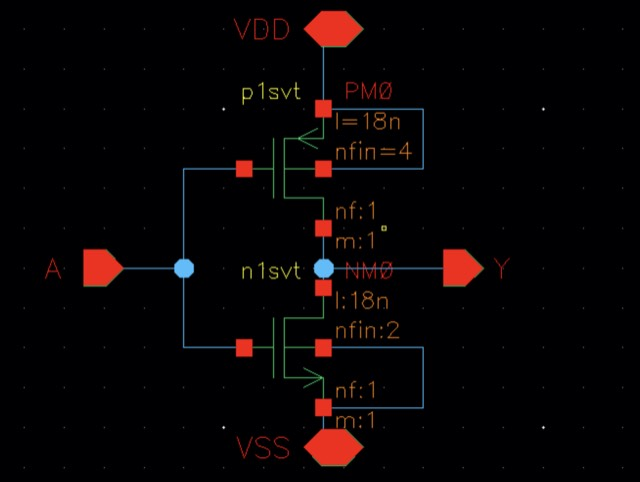
\includegraphics[width=\linewidth]{inv_u_schematic}\caption{\code{inv\_u}}\end{subfigure}\hfill
\begin{subfigure}{.19\linewidth}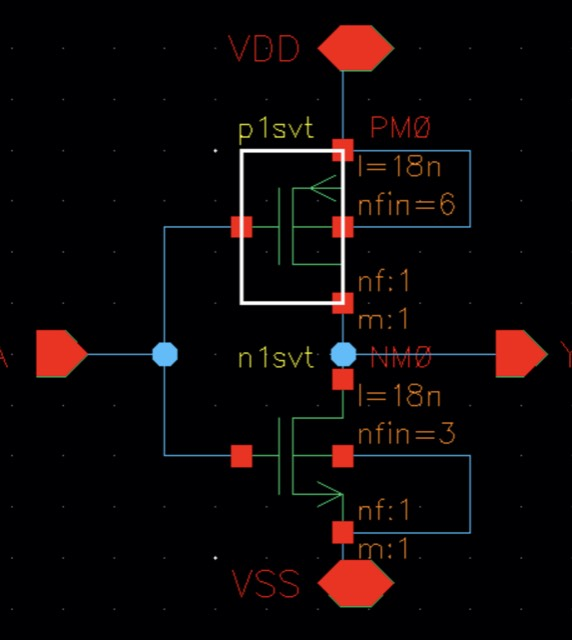
\includegraphics[width=\linewidth]{inv_drv_schematic}\caption{\code{inv\_drv}}\end{subfigure}\hfill
\begin{subfigure}{.19\linewidth}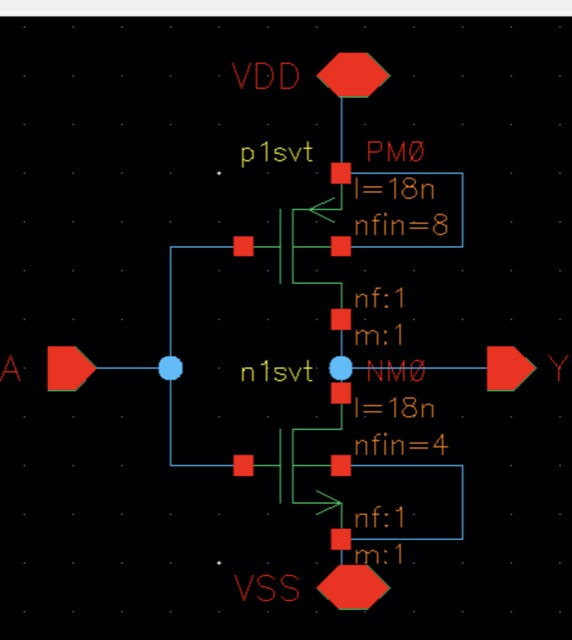
\includegraphics[width=\linewidth]{inv_2x_schematic}\caption{\code{inv\_2x}}\end{subfigure}\hfill
\begin{subfigure}{.19\linewidth}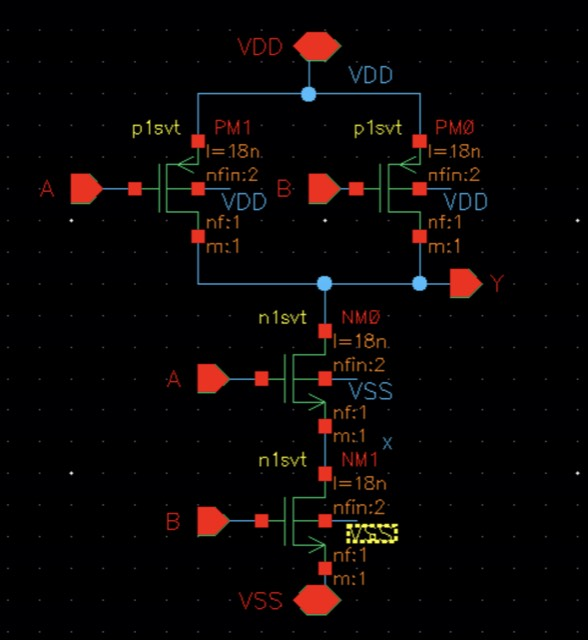
\includegraphics[width=\linewidth]{nand2_u_schematic}\caption{\code{nand2\_u}}\end{subfigure}\hfill
\begin{subfigure}{.19\linewidth}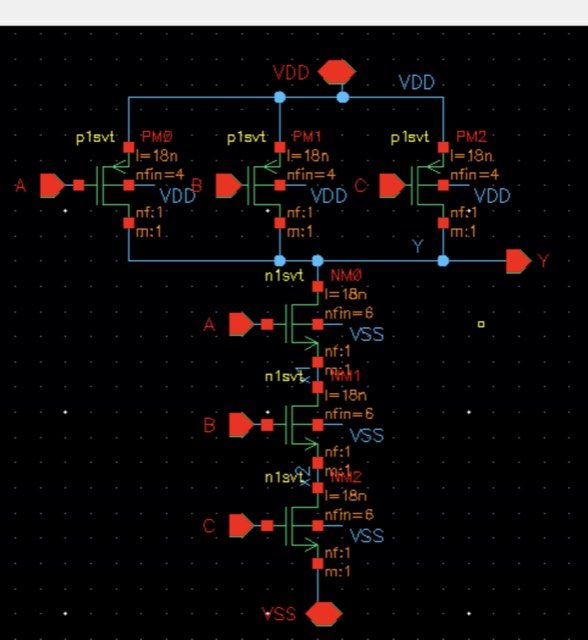
\includegraphics[width=\linewidth]{nand3_u_schematic}\caption{\code{nand3\_u}}\end{subfigure}
\caption{Decoder gates with sizes.}\end{figure}
\fig{decoder_predec_schematic}{.8}{\code{decoder\_predec}: predecode gates (top and middle) and the 16 \code{row\_pre} instances.}

\textbf{Logical effort} (address$\to$WL, 4 gates: \code{nand3\_u}, \code{inv\_2x}, \code{nand2\_u}, \code{inv\_drv}). Assumptions: $\tau=10.5$ ps (FO4 $=5\tau$, below), $\approx20$ aF of gate capacitance per fin (Part 1: 90 aF per cell over 4 pass-gate fins), $p_{\text{INV}}=1$, $p_{\text{NAND2}}=2$, $p_{\text{NAND3}}=3$, $C_{WL}=0.5$ fF. $G=\tfrac53\cdot1\cdot\tfrac43\cdot1=\tfrac{20}9=2.2$; each literal reaches 2 predecode gates and each predecode output drives 4 rows, $B=2\times4=8$; $C_{in}=10$ fins $=200$ aF (one \code{nand3\_u} input), so $H=500/200=2.5$ and $F=GBH=44$; $\hat N=\log_4F=2.7$; at the 4 stages used the stage effort is $F^{1/4}=2.6$ (below the optimum of $\approx4$, so the 4 stages are not buffer-limited); $P=3+1+2+1=7$; $D=4(2.6)+7=17.3\,\tau\approx182$ ps. This predicts the address-to-wordline path ($B=8$ is the fan-out of an address literal). Measured below, with WL\_EN held high and $A\langle0\rangle$ switching (PA path): 106 ps for the new row rising and 112 ps for the old row falling, so the model overestimates by about $1.6\times$ (182 vs.\ 112 ps). The 97 ps WL\_EN-to-wordline delay is a different path and is not compared with the prediction.

\textbf{FO4 delay.} Chain of \code{inv\_u} (\code{tb\_fo4}), 0.4 V crossings: $t_{pHL}=54.7$ ps, $t_{pLH}=50.6$ ps, FO4 $=52.6\approx53$ ps; $\tau=10.5$ ps \est.
\fig{tb_fo4_tran}{.6}{\code{tb\_fo4}: IN, N1, N2 for a chain of \code{inv\_u}.}

\textbf{Measured decoder delay} (\code{tb\_dec\_pre}, 0.5 fF per wordline, WL\_EN 300 ps with 20 ps edges, static address): WL\_EN$\to$WL rising 97.4 ps, falling 101 ps, identical at all 16 addresses (the enable always enters the same \code{nand3\_u} pin). The peak of the summed wordlines is 824 mV at every address, i.e.\ exactly one wordline high ($<1$ V) and it reaches high ($>0.72$ V). \code{wl\_idx} (row index weighted by wordline peak, over 0.824 V) returns the selected row:
\begin{center}\scriptsize\setlength{\tabcolsep}{3pt}\begin{tabular}{l|cccccccccccccccc}\toprule Address & 0&1&2&3&4&5&6&7&8&9&10&11&12&13&14&15\\\midrule
\code{wl\_idx} & 0.059&1.061&2.063&3.064&4.034&5.035&6.037&7.039&8.009&9.01&10.01&11.01&11.98&12.98&13.99&14.99\\\bottomrule\end{tabular}\end{center}
Each value is distinct and within 0.07 of its row (offsets are coupling glitches of about 2 mV on rows sharing PA$\langle0\rangle$, weighted by row number: $(4+8+12)\times2$ mV$/0.824$ V $=0.058$ vs.\ 0.059 at address 0). So each address selects its own row.
\fig{tb_dec_pre_tran_addr0}{.8}{Address 0: only WL$\langle0\rangle$ rises; other rows show $\le2$ mV coupling.}

\textbf{Address-to-wordline delay (2.2a) and alternatives (2.2b).} With WL\_EN held high and $A\langle0\rangle$ switching with its complement (the PA path, 0.5 fF per wordline), the address-to-wordline delay is 106 ps for the new row rising and 112 ps for the old row falling, against 182 ps predicted with $B=8$: the logical-effort model overestimates by about $1.6\times$. The old and new rows overlap briefly (summed peak 1.02 V, above the 1 V limit of the static test), which is why the wordlines are gated by WL\_EN; the falling WL\_EN delay is not defined here because WL\_EN does not switch.
\fig{tb_dec_pre_addr_to_wl}{.8}{Address-to-wordline delay: $A\langle0\rangle$ switches with WL\_EN held high; WL$\langle1\rangle$ rises 106 ps after the new address and WL$\langle0\rangle$ falls 112 ps after it.}
\todo{Repeat with $A\langle2\rangle$ (the PB path) and quote the slower; then the flat design (4-input NAND per row; WL\_EN enters at the row NAND2, two stages from the wordline, so compare address-to-wordline for both decoders): logical effort, simulated delay, and the comparison.}

%==============================================================
\section*{4. Timing and controller (2.2c, 2.4)}
\rub{1.5 pt}{derived WL pulse widths; annotated timing diagram; controller schematic; margin analysis, incl.\ recovery if $C_{BL}$ is 20\% larger. \textbf{Status: partial.}}

\textbf{Derived pulse widths (2.2c).}
\begin{center}\small\begin{tabular}{lll}\toprule Quantity & Value & Source\\\midrule
Bitline reaches the read inverter's trip point & 83 ps & read-column test (\S5)\\
Read: minimum WL pulse (50\% width) & $\approx110$ ps & 83 ps plus margin \est\\
Write: minimum WL pulse (50\% width) & 100 to 120 ps & write-driver sweep (\S5)\\
Design WL pulse (50\% width) & 140 ps & set by the write\\\bottomrule\end{tabular}\end{center}
At $+20\%$ $C_{BL}$ the bitline time scales to $\approx100$ ps \est, inside 140 ps; the write sets the pulse.
\begin{figure}[H]\centering\resizebox{\linewidth}{!}{% Annotated timing diagram for 2.2c (TikZ). Needs \usepackage{tikz} and \usetikzlibrary{arrows.meta}.
% Times in ps from the rising CLK edge (clock period 1 ns, CLK falls at 500 ps).
% Measured: CLK->WL 238, WL->RD_EN 96, RD_EN width 136, WL fall before PRE_B fall 157,
% RD_EN fall before PRE_B fall 70, PRE_B rise before WR_EN rise 155, t_blb 83, t_wr ~96, access 226 from WL.
% Derived from these: WL fall = 540-157 = 383; RD_EN = 334..470; PRE_B edges follow CLK by ~40 ps;
% WR_EN width taken equal to WL_EN width (~134 ps, not measured).
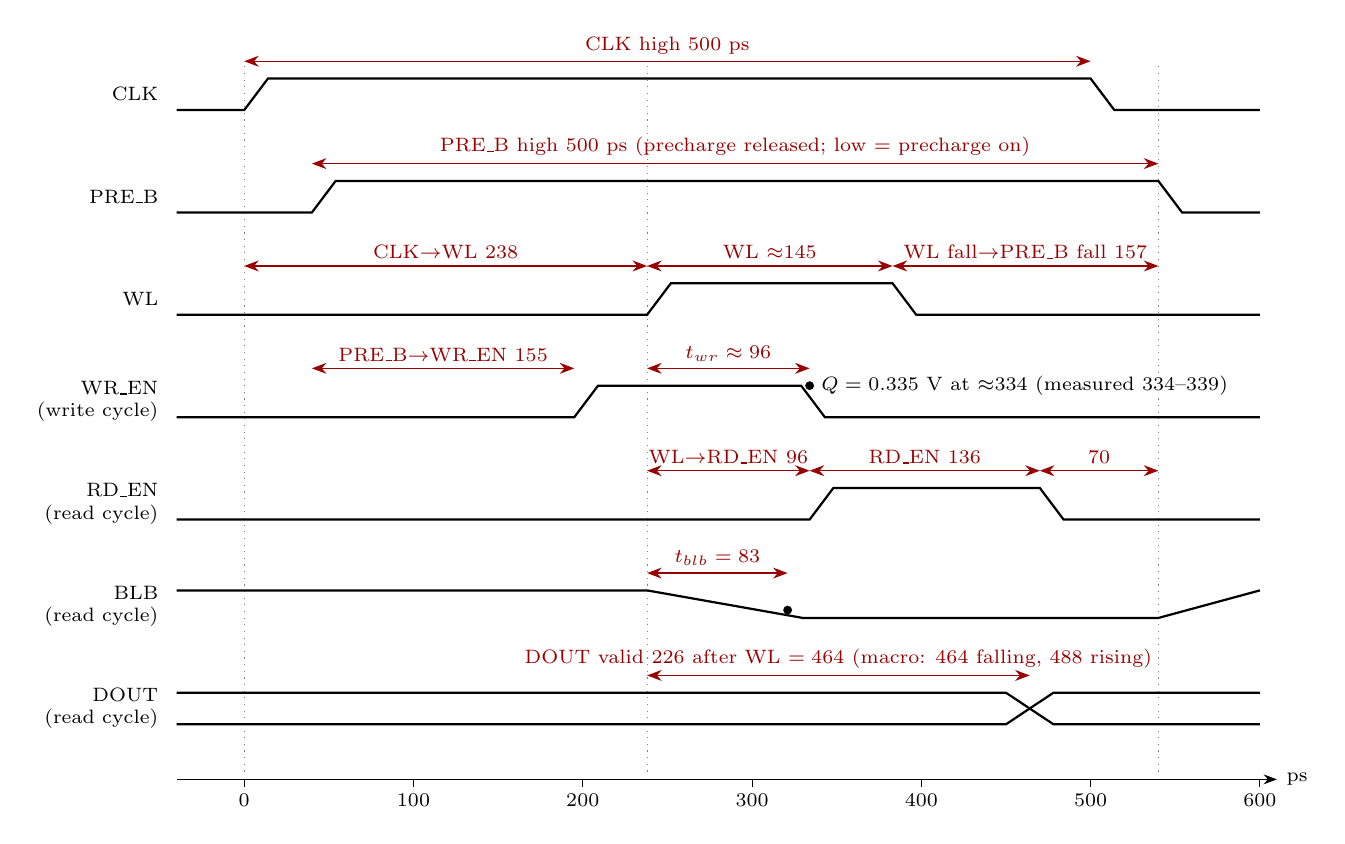
\begin{tikzpicture}[x=0.0215cm,y=1cm,font=\scriptsize,>=Stealth]
\tikzset{sig/.style={thick},dm/.style={<->,red!60!black,line width=.5pt},guide/.style={dotted,gray}}
\newcommand{\pulse}[3]{\draw[sig] (-40,#1)--(#2,#1)--({#2+14},{#1+.4})--(#3,{#1+.4})--({#3+14},#1)--(600,#1);}
\newcommand{\dm}[5]{\draw[dm] (#2,#1)--(#3,#1) node[midway,above=-1pt,#5]{#4};}
% guides
\draw[guide] (0,-.4)--(0,8.6); \draw[guide] (238,-.4)--(238,8.6); \draw[guide] (540,-.4)--(540,8.6);
% signals (low level y0, high level y0+.4)
\node[anchor=east] at (-45,8.2) {CLK}; \pulse{8}{0}{500}
\node[anchor=east] at (-45,6.9) {PRE\_B}; \pulse{6.7}{40}{540}
\node[anchor=east] at (-45,5.6) {WL}; \pulse{5.4}{238}{383}
\node[anchor=east,align=right] at (-45,4.3) {WR\_EN\\(write cycle)}; \pulse{4.1}{195}{329}
\node[anchor=east,align=right] at (-45,3.0) {RD\_EN\\(read cycle)}; \pulse{2.8}{334}{470}
\node[anchor=east,align=right] at (-45,1.7) {BLB\\(read cycle)};
\draw[sig] (-40,1.9)--(238,1.9)--(330,1.55)--(540,1.55)--(600,1.9);
\node[anchor=east,align=right] at (-45,.4) {DOUT\\(read cycle)};
\draw[sig] (-40,.6)--(450,.6)--(478,.2)--(600,.2); \draw[sig] (-40,.2)--(450,.2)--(478,.6)--(600,.6);
% dimensions
\dm{8.62}{0}{500}{CLK high 500 ps}{}
\dm{7.32}{40}{540}{PRE\_B high 500 ps (precharge released; low $=$ precharge on)}{}
\dm{6.02}{0}{238}{CLK$\to$WL 238}{}
\dm{6.02}{238}{383}{WL $\approx$145}{}
\dm{6.02}{383}{540}{WL fall$\to$PRE\_B fall 157}{}
\dm{4.72}{40}{195}{PRE\_B$\to$WR\_EN 155}{}
\dm{4.72}{238}{334}{$t_{wr}\approx96$}{}
\dm{3.42}{238}{334}{WL$\to$RD\_EN 96}{}
\dm{3.42}{334}{470}{RD\_EN 136}{}
\dm{3.42}{470}{540}{70}{}
\dm{2.12}{238}{321}{$t_{blb}=83$}{}
\dm{.82}{238}{464}{DOUT valid 226 after WL $=464$ (macro: 464 falling, 488 rising)}{}
% markers
\fill (334,4.5) circle (1.6pt) node[right=3pt,fill=white,inner sep=1pt] {$Q=0.335$ V at $\approx$334 (measured 334--339)};
\fill (321,1.65) circle (1.6pt);
% time axis
\draw[->] (-40,-.5)--(610,-.5) node[right] {ps};
\foreach \t in {0,100,...,600}{\draw (\t,-.5)--(\t,-.6) node[below=-1pt]{\t};}
\end{tikzpicture}
}
\caption{Annotated timing diagram (2.2c), $t_{clk}=1$ ns, times in ps from the rising CLK edge; the WL pulse of about 145 ps exceeds the minimum read (110) and write (100 to 120) pulses. Measured: CLK$\to$WL 238, WL$\to$RD\_EN 96, RD\_EN width 136, WL and RD\_EN fall 157 and 70 ps before PRE\_B falls, PRE\_B rises 155 before WR\_EN, $t_{blb}=83$, write time $\approx96$ after WL, access 226 after WL. Derived from these: WL fall at $540-157=383$ ps; RD\_EN from 334 to 470 ps; PRE\_B edges $\approx40$ ps after CLK; the WR\_EN width is taken equal to WL\_EN's (not measured). BLB is a sketch (not to voltage scale). PRE\_B low turns the precharge on, so the bitlines are released at the rising edge and recharge from 540 ps.}\end{figure}

\textbf{Controller (2.4).} Inputs CLK, WE, ADDR, DIN; outputs A, AB, D, PRE\_B, WL\_EN, WR\_EN, RD\_EN. Input latches (\code{out\_latch}, enable CLKBL from its own \code{inv\_2x}) hold ADDR, DIN, WE while CLK is high. PRE\_B $=$ \code{inv\_2x}(CLKB) follows CLK; the precharge cell is three PMOS gated by PRE\_B, so precharge is on while CLK is low. WL\_EN $=$ CLKBUF AND (CLKBUF through 7 \code{inv\_u}): a one-shot per rising edge. WR\_EN $=$ WL\_EN AND WE; RD\_EN $=$ (WL\_EN through 8 \code{inv\_u}) AND $\overline{\text{WE}}$.
\fig{controller_schematic}{.85}{\code{controller}: input latches, WL\_EN one-shot (DLY1), WR\_EN and RD\_EN (DLY2).}
\begin{center}\small\begin{tabular}{lrrl}\toprule \code{tb\_controller} (0.4 V crossings) & Before & After & Note\\\midrule
CLK $\to$ WL (\code{t\_clk\_wl}) & 356 ps & 238 ps & latch enable moved to own inverter\\
RD\_EN fall before PRE\_B fall (\code{m\_rd\_pre}) & 30 ps & 70 ps & smallest margin\\
WL fall before PRE\_B fall (\code{m\_wl\_pre}) & 118 ps & 157 ps & \\
PRE\_B rise before WR\_EN rise (\code{gap\_pre\_wr}) & 178 ps & 155 ps & \\
WL $\to$ RD\_EN (\code{t\_wl\_rden}) & 96 ps & 96 ps & column test needs $\ge80$\\
RD\_EN width (\code{rden\_w}) & 136 ps & 136 ps & column test needs $\ge100$\\
WL\_EN width (\code{wlen\_w}) & 134 ps & 134 ps & write needs 120 to 140\\\bottomrule\end{tabular}\end{center}
Margin on each edge (after): WL\_EN width $+14$ ps over 120 ps; RD\_EN lead $+16$ ps over 80 ps; RD\_EN width $+36$ ps over 100 ps; RD\_EN before precharge $+70$ ps; WL before precharge $+157$ ps; PRE\_B before WR\_EN $+155$ ps. No spurious pulses: RD\_EN peaks at 3.3 mV in a write cycle and WR\_EN at 0.41 mV in a read cycle ($<80$ mV).
\fig{tb_controller_tran}{.85}{Controller transient: WR\_EN pulses only in write cycles, RD\_EN only in read cycles; WL ends before PRE\_B falls.}
\textbf{Limit and recovery.} The 70 ps RD\_EN margin does not set $T_{CLK,\min}$: it was estimated to vanish near 0.86 ns, yet the macro passes down to 0.69 ns (\S6, \S7). The edge that fails below 0.69 ns is not identified. If $C_{BL}$ were 20\% larger the read delays grow, and the recovery is a shorter DLY2 chain or a longer clock half period. \textit{The controller bench has no bitlines, so its loads do not model a larger $C_{BL}$; the pulses stay fixed and the column timing moves relative to them.} \todo{Test $+20\%$ $C_{BL}$ in a bench with real bitlines: the macro run with \code{cbw} $=1.32$ fF, or \code{tb\_read\_col} with $C_{BL}=4.2$ fF, and report the margin on each edge.}

%==============================================================
\section*{5. Column circuits and unit tests (2.3)}
\rub{(within the 1.5 pt controller/column item)}{precharge, write driver, read path (state the differential and margin), output latch, each unit-tested. \textbf{Status: done} at $C_{BL}=3.5$ fF stand-in; \todo{rerun with the extracted $C_{BL}$}.}

\fig{sram_col_schematic}{.62}{\code{sram\_col} (one per bit): precharge (I1), write driver (I2), read path (I3), output latch (I4), the 16 cells \code{X<15:0>}, and the wire capacitance \code{cbw} on BL and BLB.}
\code{sram\_col} has no standalone bench: \code{tb\_read\_col} (below) tests the same four circuits on one cell with $C_{BL}$ on both bitlines, and \code{sram\_col} itself is verified in \code{tb\_sram\_macro} (four instances, all 16 rows, tests (i) and (ii)) and \code{tb\_sram\_macro\_t3} (test (iii)), \S6.

\textbf{Precharge:} three PMOS (2 fins each: one per bitline to VDD, one equalizer), gate PRE\_B. Recovery at $C_{BL}=3.5$ fF: BL reaches 99\% of $V_{DD}$ in 142 ps, with a peak of 845 mV and BLB near 690 mV during equalization.
\fig{precharge_schematic}{.35}{\code{precharge}.}

\textbf{Write driver} (36 fins: four 8-fin NMOS pull-downs plus a 2+2-fin inverter). A small driver fails because the write races an undriven bitline: the cell discharges BLB through its pass gate, pinning QB low and blocking the cell's feedback. Fin sweep, pulse 0.3 ns, $C_{BL}=3.5$ fF:
\begin{center}\small\begin{tabular}{rlrrr}\toprule nfin & Write 0 & $t_{wr0}$ & $t_{wr1}$ & lowest BLB (mV, from waveform)\\\midrule
2 & fail, Q stalls at 0.66 V & -- & -- & $\sim0$\\ 4 & fail, Q stalls at 0.38 V & -- & -- & $\sim60$\\ 5 & pass & 153 ps & 154 ps & $\sim190$\\ 6 & pass & 121 ps & 121 ps & $\sim260$\\ \textbf{8} & pass & 96 ps & 96 ps & $\sim345$\\\bottomrule\end{tabular}\end{center}
\begin{center}\small\begin{tabular}{rll}\toprule \code{pw\_w1} (WL at 50\% $=+20$ ps) & $C_{BL}=3.5$ fF & $4.2$ fF ($+20\%$)\\\midrule
40p, 60p, 80p & fail (Q stalls 0.62, 0.46, 0.27 V) & fail (0.66, 0.51, 0.34 V)\\ 100p, 120p, 150p & pass, 96 ps & pass, 102 ps\\\bottomrule\end{tabular}\end{center}
nfin 5 is the smallest that writes; nfin 8 is provisional (6 vs.\ 8 trades 0.77 $\mu$m$^2$, 3\% of the array, for 25 ps; decide with $T_{CLK,\min}$). Write time is 96 ps, 102 ps at $+20\%$ $C_{BL}$; minimum pulse 100 to 120 ps at 50\%.
\begin{figure}[H]\centering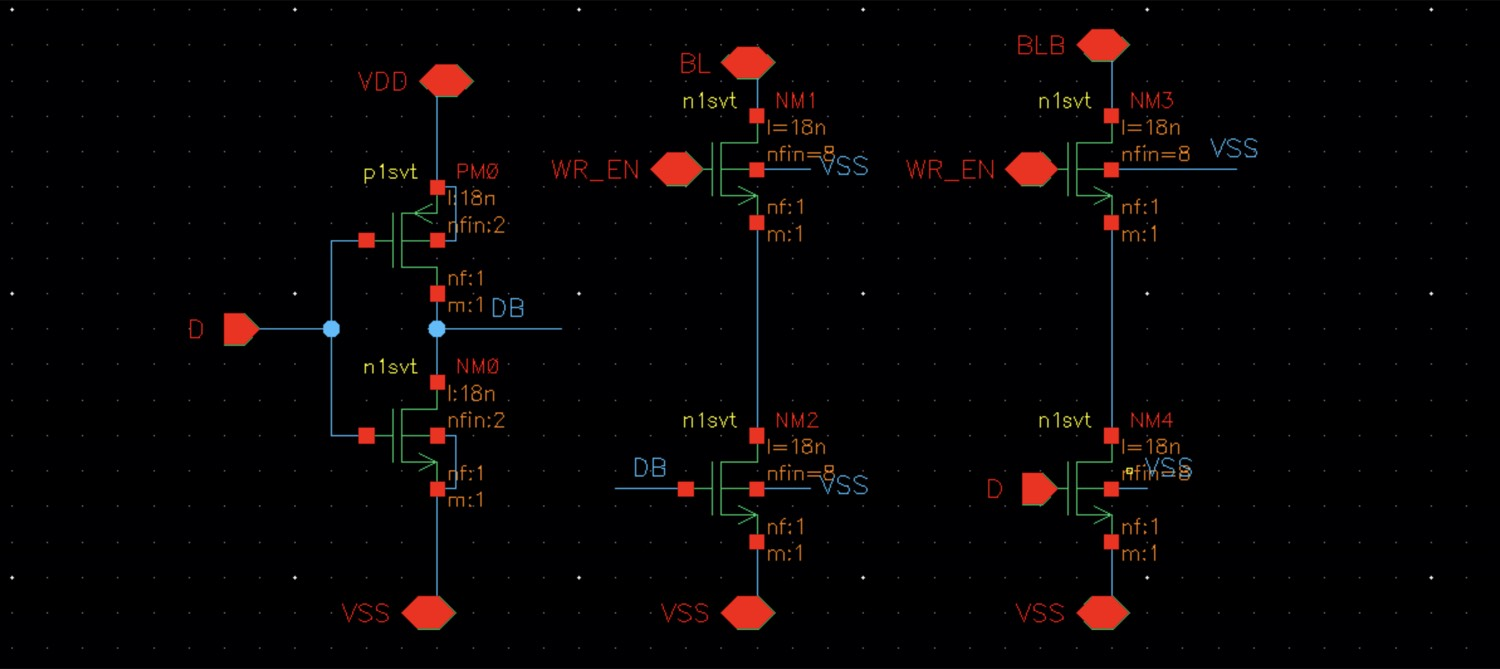
\includegraphics[width=.48\linewidth]{write_driver_schematic_nfin8}\hfill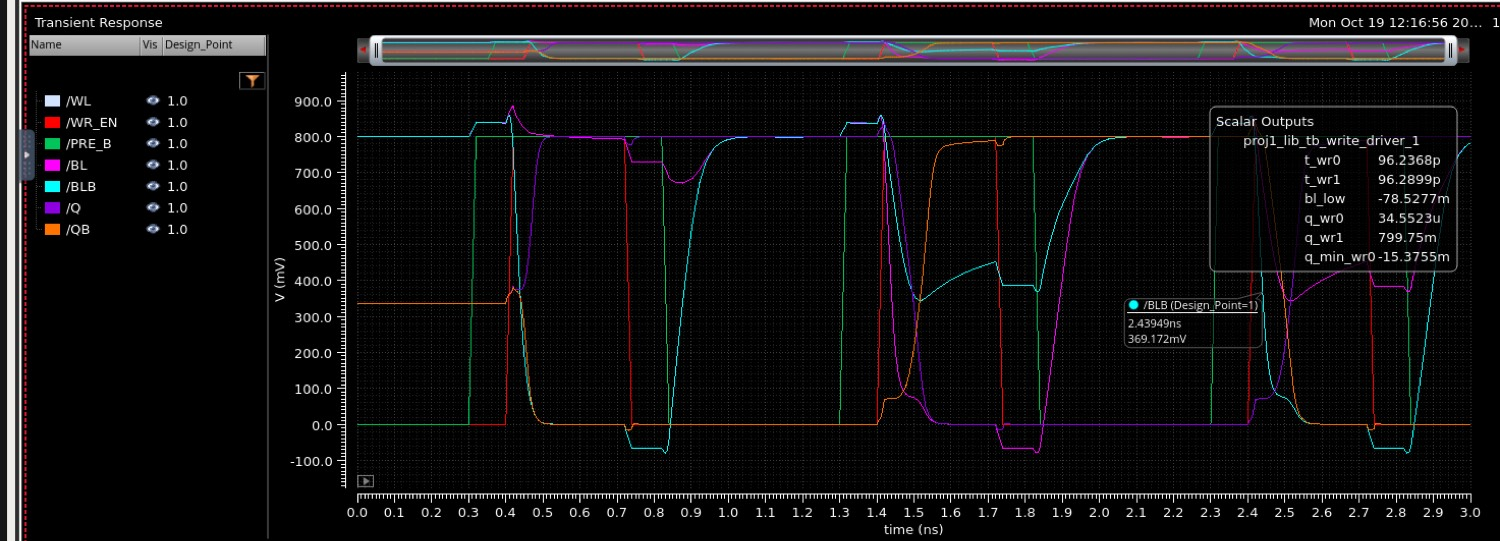
\includegraphics[width=.48\linewidth]{write_driver_tran_nfin8}\caption{Write driver at nfin 8 and its write-0/write-1 transient ($q_{wr0}=35\ \mu$V, $q_{wr1}=799.8$ mV, $t_{wr0}=96$ ps).}\end{figure}

\textbf{Read path:} inverter on BLB, full swing (no sense amplifier), sized 2:2 (PMOS 2, NMOS 2 fins), switching point 0.376 V, i.e.\ BLB must fall $0.8-0.376=0.42$ V to flip RD (margin: the read pulse of 140 ps gives 57 ps of slack over the 83 ps bitline time). 4:2 would switch at 0.415 V, save $\approx7$ ps \est\ and add 8 fins ($0.19\ \mu$m$^2$); it is not on the critical path since the write sets the pulse.
\begin{figure}[H]\centering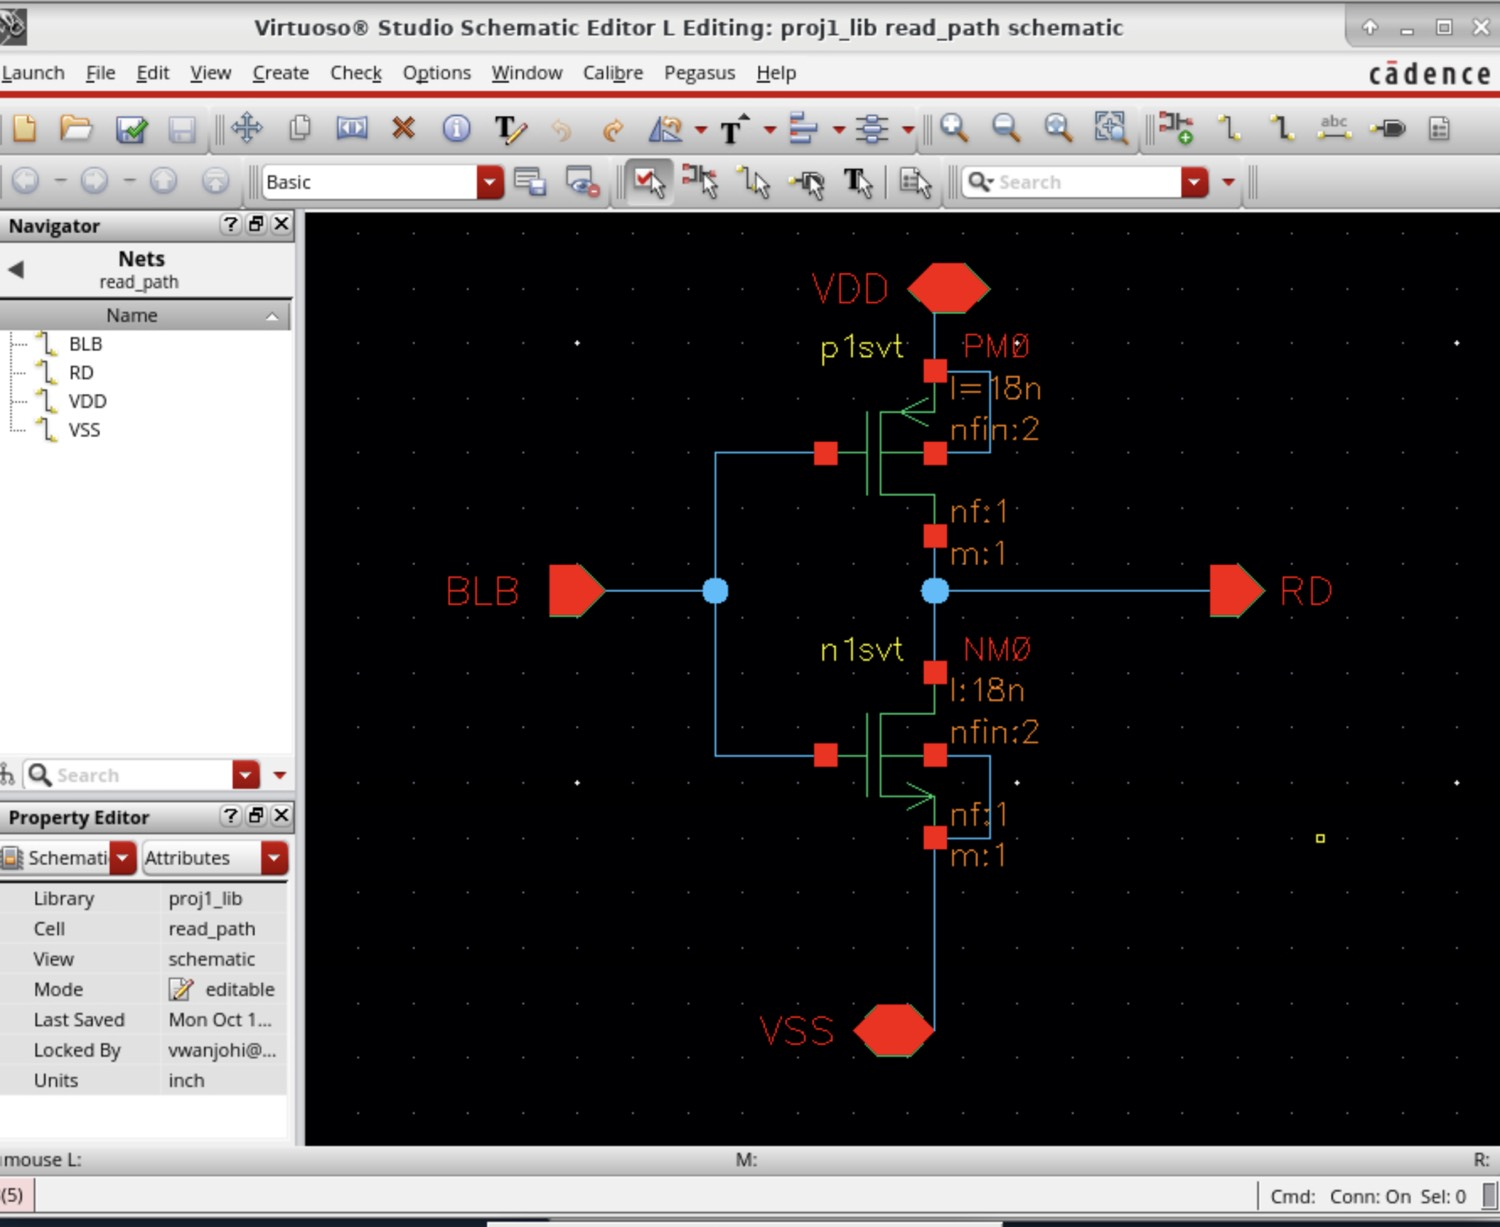
\includegraphics[width=.4\linewidth]{read_path_schematic_library_view_2to2}\hfill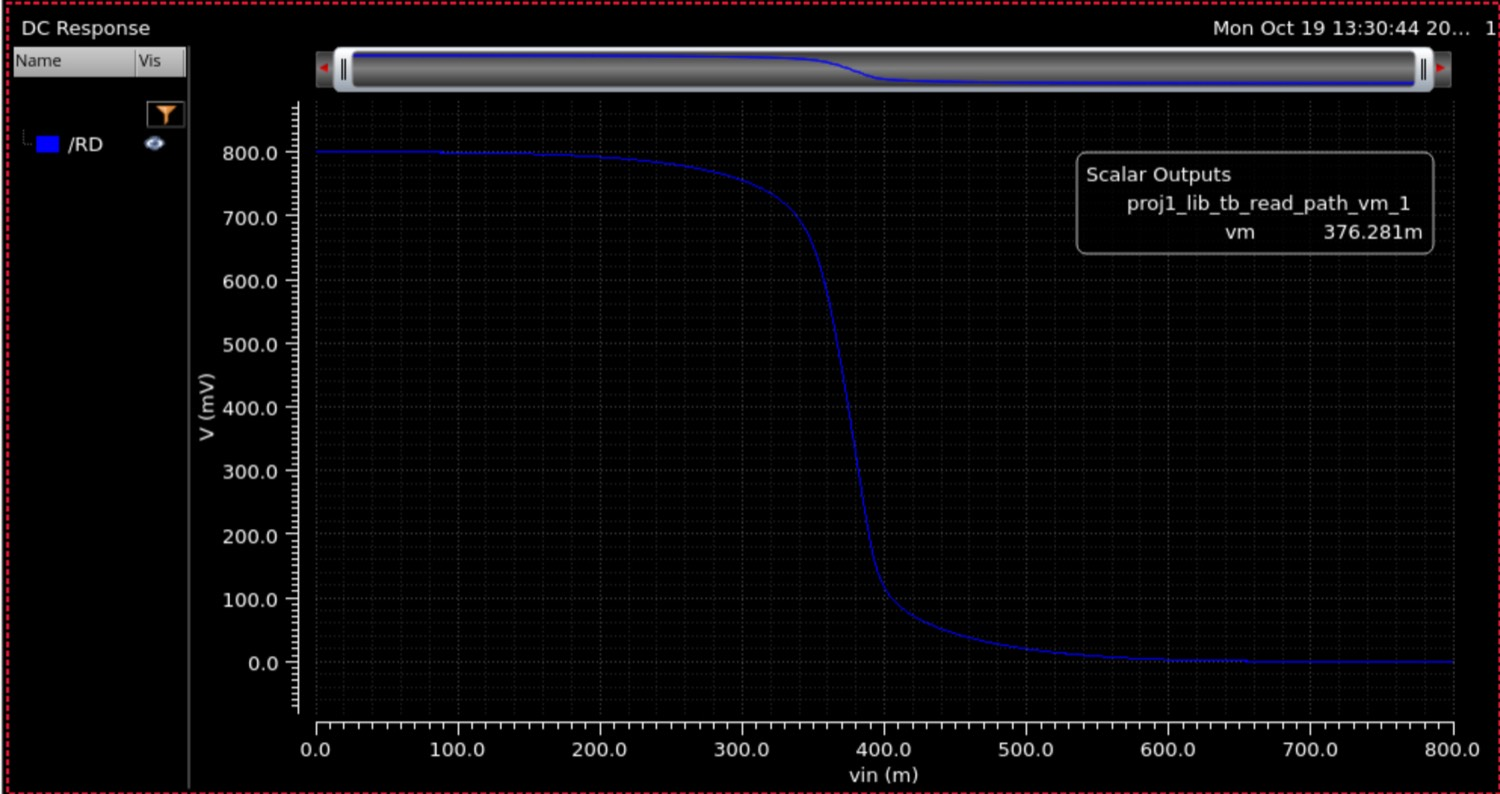
\includegraphics[width=.55\linewidth]{read_path_vtc_2to2}\caption{\code{read\_path} (2:2) and its transfer curve, $V_M=376$ mV.}\end{figure}

\textbf{Output latch} (all devices 2 fins, 24 fins). Enable-pulse sweep ($c_{dout}=1$ fF; specs hold-1 $>0.72$ V, hold-0 $<0.08$ V):
\begin{center}\small\begin{tabular}{rrrrrl}\toprule \code{pw\_en} & $t_{en,r}$ & $t_{en,f}$ & hold-1 & hold-0 & \\\midrule
10p & -- & -- & $-58\ \mu$V & 77 $\mu$V & fail\\ 20p & 99.5 ps & 76.0 ps & 799.8 mV & 88 $\mu$V & pass\\ 40p & 88.7 ps & 74.8 ps & 799.8 mV & 89 $\mu$V & pass\\ 80p & 87.2 ps & 74.5 ps & 799.8 mV & 125 $\mu$V & pass\\ 150p & 87.3 ps & 74.5 ps & 799.2 mV & 1.25 mV & pass\\\bottomrule\end{tabular}\end{center}
\begin{figure}[H]\centering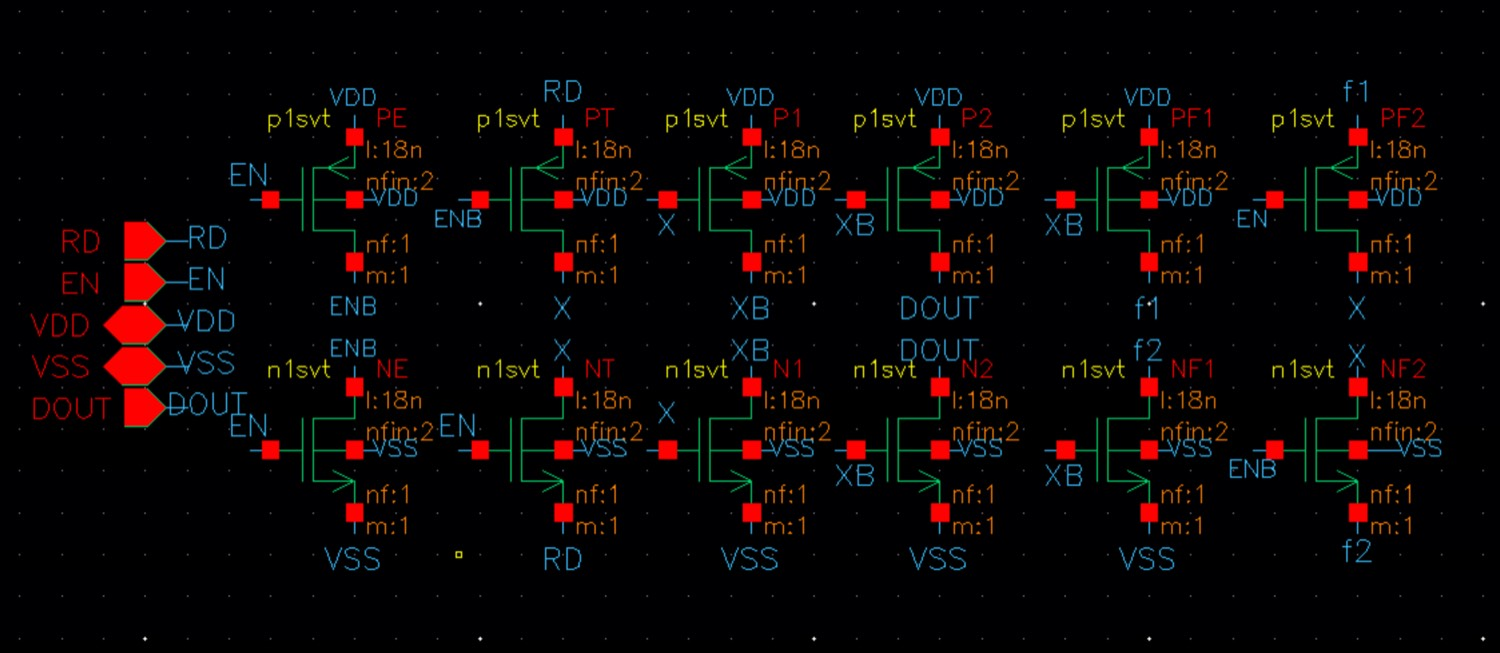
\includegraphics[width=.34\linewidth]{out_latch_schematic}\hfill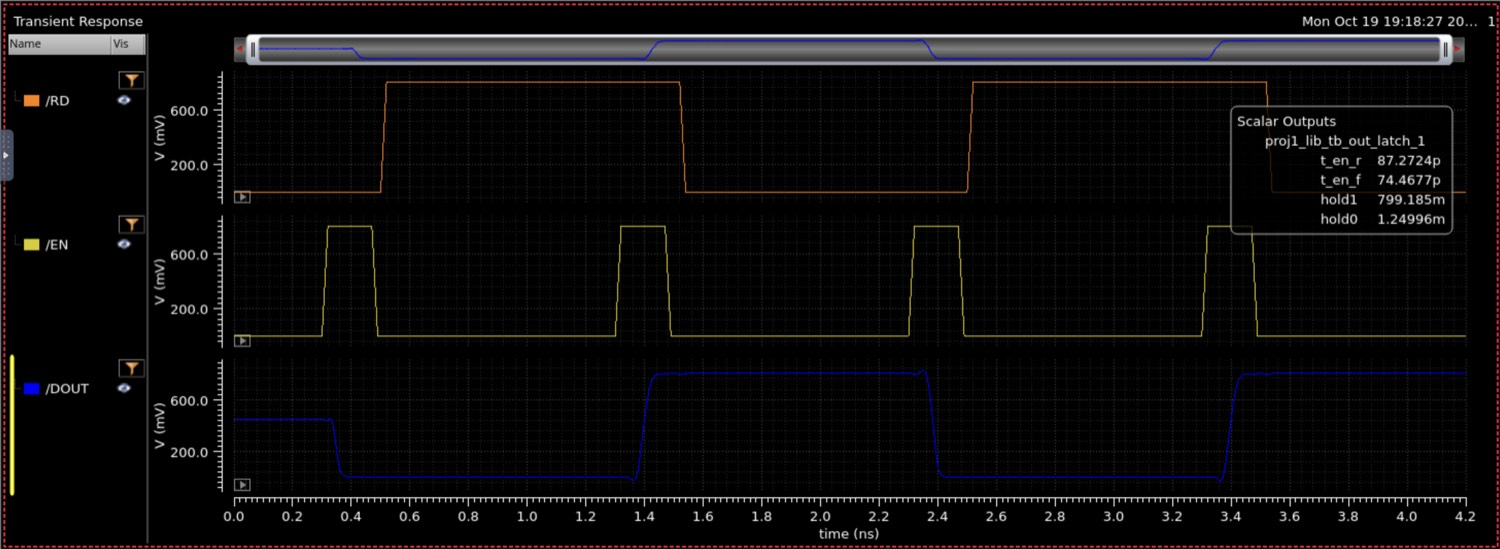
\includegraphics[width=.62\linewidth]{out_latch_tran_en_delay300p}\caption{\code{out\_latch} and its unit test at 150 ps (DOUT written only while EN is high).}\end{figure}

\textbf{Read column} (cell, write driver, precharge, read path, latch; write 1, read, write 0, read, write 1, read). Read-1 access $t_{acc1}$ (WL$\to$DOUT, ps) over latch-enable delay \code{rd\_dly} and width \code{pw\_rden} (24 points); all checks pass except the third read at \code{pw\_rden}\,$=40$ p (latch never captures the 1):
\begin{center}\small\begin{tabular}{rrrrrr}\toprule \code{rd\_dly} & 40p & 80p & 120p & 160p & $t_{acc0}$\\\midrule
1.48n & fail & 247 & 226 & 226 & 165\\ 1.52n & fail & 235 & 235 & 235 & 205\\ 1.56n & fail & 271 & 271 & 271 & 245\\ 1.60n & fail & 311 & 311 & 311 & 285\\ 1.64n & fail & 351 & 351 & 351 & 325\\ 1.68n & fail & 391 & 391 & 391 & 365\\\bottomrule\end{tabular}\end{center}
Opening the latch later only adds delay (40 ps per 40 ps of \code{rd\_dly}). \textbf{Chosen: \code{rd\_dly}\,$=1.48$ n, \code{pw\_rden}\,$=120$ p} (shortest width that loses nothing): BLB reaches the read inverter's switching point 83 ps after WL, RD crosses 0.4 V at 113 ps (140 ps with the latch loading it), DOUT valid 165 ps (read 0) and 226 ps (read 1) after WL; the cell is undisturbed ($q_{rd1}=799.7$ mV, $q_{rd0}=39\ \mu$V).
\fig{read_col_tran_1p48n_120p_zoom_read3_stacked_BEST}{.9}{Cycle 6 read of a 1, $C_{BL}=3.5$ fF, \code{rd\_dly}\,$=1.48$ n, \code{pw\_rden}\,$=120$ p: BLB crosses the read inverter's 0.376 V switching point 83 ps after WL rises; DOUT is valid 226 ps after WL rises.}

%==============================================================
\section*{6. Verification (2.5)}
\rub{1 pt}{full-macro checkerboard write/read, complement overwrite/read, worst-case-row read-after-write; waveforms for (iii), pass/fail table for (i)--(ii); inputs through realistic buffers. \textbf{Status: done.}}

\textbf{Bench} (\code{tb\_sram\_macro}, $t_{clk}$ swept, DOUT loaded by 1 fF): CLK, WE and ADDR pass through two \code{inv\_u} stages each. The address is a binary counter (one step per cycle); WE is high for 16 cycles (write all words), then low for 16 (read all), repeating. DIN $=\{X,\bar X,X,\bar X\}$ with $X=a_0\oplus ph$: each word is 0101 or 1010 alternating by row, and $ph$ flips at $32.25\,t_{clk}$ to complement every word. Checks: \code{err1} (checkerboard read pass) and \code{err2} (complement read pass), each the maximum DOUT error over the read window against 0.1 V; \code{err3} is test (iii).
\fig{tb_sram_macro_buffers_and_data_gates}{.85}{Input buffers (IB1, IB2) and the NAND XOR that builds the DIN pattern.}
\begin{center}\small\begin{tabularx}{\linewidth}{@{}p{.3\linewidth}Xl@{}}\toprule Test & Result at $t_{clk}=1$ ns & \\\midrule
(i) checkerboard write, read all 16 & \code{err1} $=173.8\ \mu$V ($<0.1$ V) & \textbf{pass}\\
(ii) complement overwrite, read all 16 & \code{err2} $=173.8\ \mu$V & \textbf{pass}\\
(iii) far-end row (row 15), read right after a write to the opposite value & \code{err3} $=173.8\ \mu$V & \textbf{pass}\\\bottomrule\end{tabularx}\end{center}
\fig{tb_sram_macro_tran_dout}{.85}{DOUT$\langle3{:}0\rangle$: bits 3,1 opposite to bits 2,0 (0101/1010 alternating each cycle); DOUT holds while WE is high (32 to 49 ns).}
\begin{figure}[H]\centering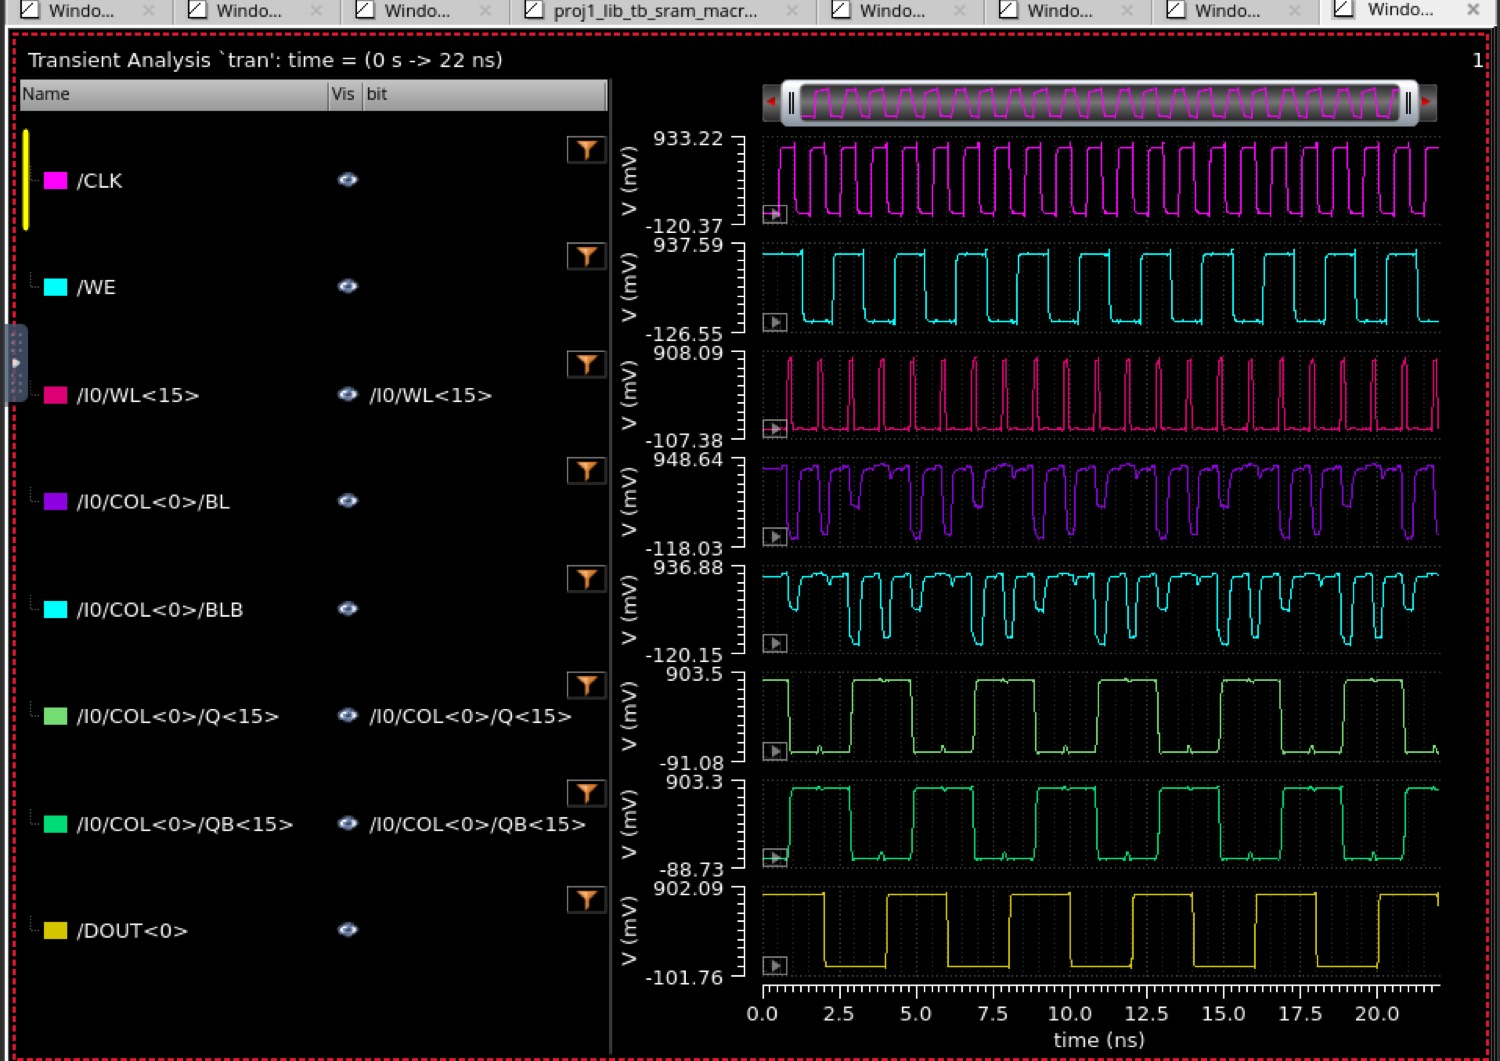
\includegraphics[width=.57\linewidth]{tb_sram_macro_row15_all_signals_22ns_BEST}\hfill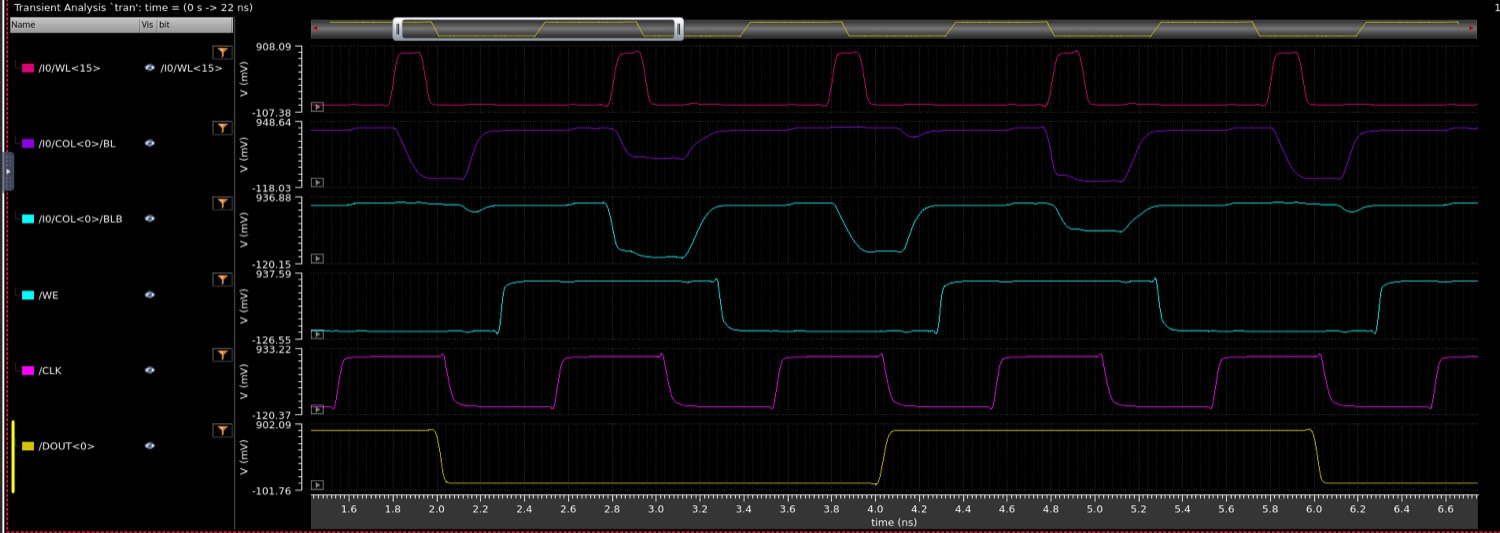
\includegraphics[width=.4\linewidth]{tb_sram_macro_row15_wl_bl_we_clk_dout_zoom_BEST}\caption{Test (iii), row 15 (the far-end row, a stand-in: at schematic level all rows are equivalent): WE alternates every cycle; each read returns the value just written, which is the opposite of the previous one. DOUT changes only after the reads (about 0.5 ns after the edge).}\end{figure}
\textbf{Write time} (later of the $Q$ and $\overline Q$ crossings of 0.335 V, from the CLK edge): 338.6 ps (write 1), 333.7 ps (write 0); the cursors give 333.3 ps (CLK 448 mV to $Q$ 306 mV). \textbf{Read access} (CLK to DOUT$\langle1\rangle$, 0.4 V): 463.7 ps falling, 484.2 ps rising at 1 ns.
\fig{tb_sram_macro_write_time_markers}{.6}{Write time on row 15: cursor A at the CLK edge, cursor B on $Q\langle15\rangle$, 333.3 ps.}
\textbf{Clock-period sweep} ($t_{clk}$ from 1 ns down to 0.6 ns; power is the macro's VDD-pin current $\times0.8$ V over the write pass, read pass, and a clock-stopped window):
\begin{center}\scriptsize\setlength{\tabcolsep}{3pt}\begin{tabular}{rrrlrrrr}\toprule $t_{clk}$ & \code{err1} & \code{err2} & Result & $t_{acc,f}$ & $t_{acc,r}$ & write & read\\\midrule
700 ps & 5.10 mV & 5.12 mV & pass & 463.7 & 485.5 & 122.6 $\mu$W & 113.4 $\mu$W\\ \textbf{690 ps} & 23.3 mV & 22.4 mV & \textbf{pass} & 463.8 & 488.3 & 124.3 $\mu$W & 115.2 $\mu$W\\ 680 ps & 452 mV & 441 mV & fail & 463.8 & 496.9 & 126.0 $\mu$W & 118.0 $\mu$W\\ 670--600 ps & 1.28 V & 1.28 V & fail & 463.9--465.3 & -- & 127.7--142.8 $\mu$W & 114.9--122.8 $\mu$W\\\bottomrule\end{tabular}\end{center}
(1000 to 750 ps also pass: \code{err1}/\code{err2} grow from 174 $\mu$V to 0.50 mV; \code{err3} from 174 $\mu$V to 0.50 mV, 5.6 mV at 700 ps, about 30 mV at 690 ps, about 0.6 V at 680 ps, 1.28 V at 670 ps and below; write times stay at 338.6/333.7 ps.) Below 680 ps the read returns the wrong value (1.28 V error). $T_{CLK,\min}=0.69$ ns (10 ps resolution): 690 ps passes all three tests with about a factor of 3 of margin on \code{err3}, 680 ps fails.
\begin{figure}[H]\centering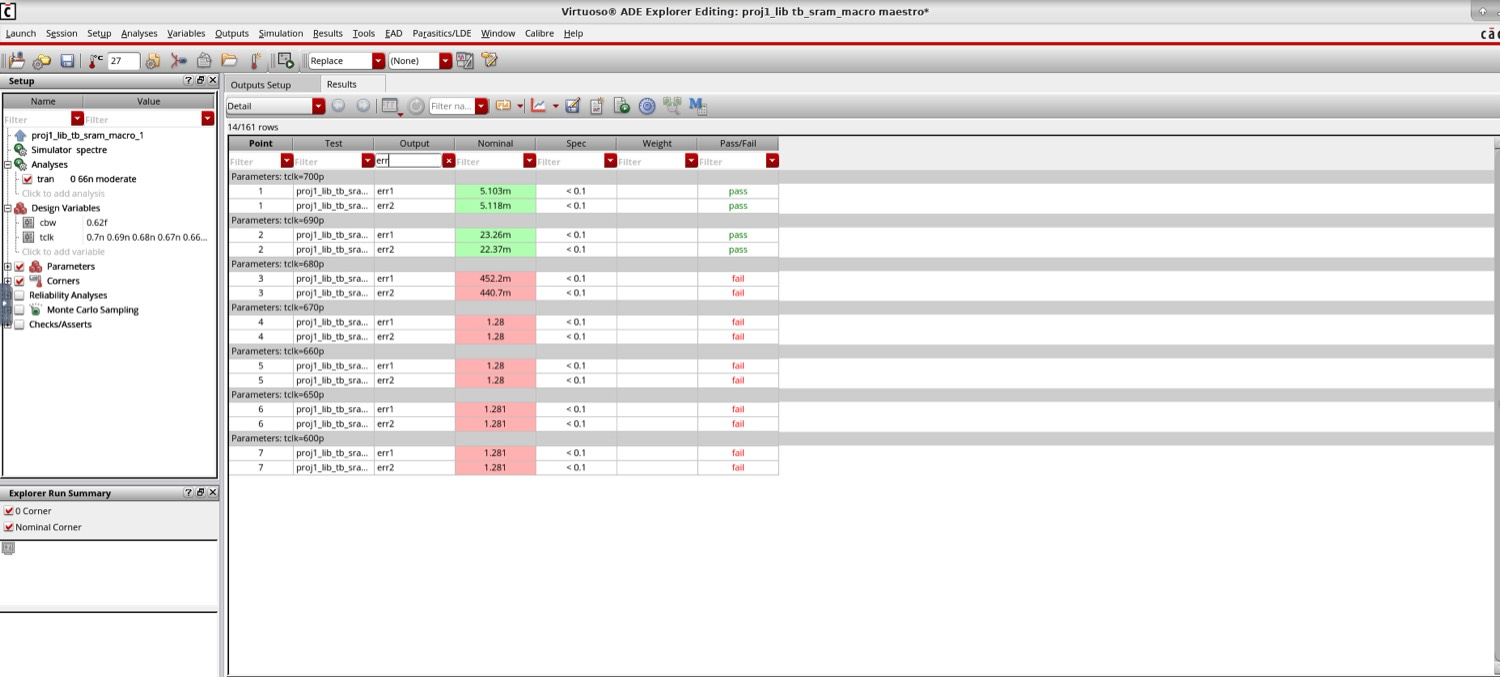
\includegraphics[width=.48\linewidth]{tb_sram_macro_tclk_600_700_err1_err2}\hfill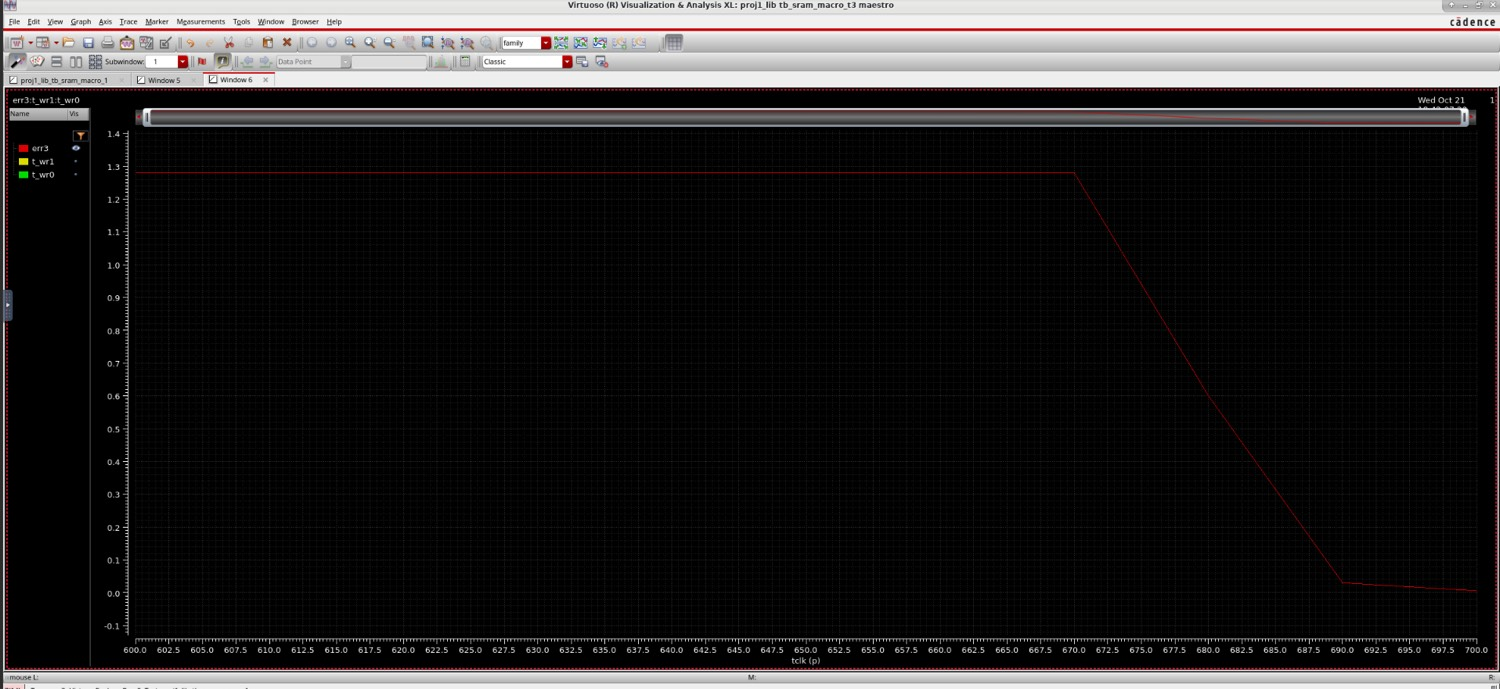
\includegraphics[width=.48\linewidth]{tb_sram_macro_tclk_sweep_err3_600_700ps}\caption{Error against clock period: \code{err1}/\code{err2} (left) and \code{err3} (right); the tests fail below 0.69 ns.}\end{figure}
\textbf{Test-bench notes.} The $a_3$ source has width $8.25\,t_{clk}-20$ ps instead of $8\,t_{clk}-20$ ps, so $a_3$ falls at the capture edge of cycle 16; the width has been corrected to $8\,t_{clk}-20$ ps in the saved bench. The results above come from the bench before the correction and are unaffected: rows 0 and 8 hold the same data, and test (iii) uses a fixed address and fails at the same period. The checks compare DOUT to a pattern that depends on $a_0$ only; correct row selection is shown by the \code{wl\_idx} test of \S3.

%==============================================================
\section*{7. Metrics and figure of merit}
\rub{(within the 1 pt verification/metrics item)}{metrics table with FOM, $D$ and $T_{CLK,\min}$. \textbf{Status: partial} (area and write power are estimates).}

At $V_{DD}=0.8$ V, nominal, 27$^\circ$C, $T_{CLK,\min}=0.69$ ns, $D=28$ ($0.39\ \mu$m$^2/(16\times0.048\times0.018\ \mu$m$^2)$):
\begin{center}\small\begin{tabular}{@{}p{.56\linewidth}p{.4\linewidth}@{}}\toprule Metric & Value\\\midrule
$T_{CLK,\min}$ & \textbf{0.69 ns} (10 ps resolution)\\
Worst-case read access (CLK to DOUT) & 488 ps at 690 ps (488.3 ps on DOUT$\langle1\rangle$, 488.9 ps on DOUT$\langle0\rangle$): the columns are identical at schematic level and the decoder delay is the same for every row, so the worst case depends on the data (a read of 1, rising output), not on the bit or the address\\
Worst-case write time (later of $Q$/$\overline Q$) & 339 ps (row 15)\\
Power, array write at $T_{CLK,\min}$ & 124.3 $\mu$W, measured with a checkerboard write pattern (second write pass), not the handout's all-0 then all-1 sequence\\
Power, checkerboard read sweep & 115.2 $\mu$W\\
Power, standby & 112.2 $\mu$W clock running (no chip-select: every edge triggers an access); 3.99 $\mu$W clock stopped (leakage)\\
Area: array (not laid out) $+$ periphery ($D\sum W_iL_i$) & $24.9+29.7=54.6\ \mu$m$^2$ \est\\
\textbf{FOM $=$ Area$\cdot$Power$\cdot T_{CLK,\min}$} & $54.6\times124.3\times0.69\approx\mathbf{4.7\times10^3}\ \mu$m$^2\cdot\mu$W$\cdot$ns \est\\\bottomrule\end{tabular}\end{center}
\fig{tb_sram_macro_sb_tran}{.6}{Standby: after the clock stops (47 ns) the macro's VDD current falls to about zero (3.99 $\mu$W).}

%==============================================================
\section*{8. Trade-offs}
\begin{itemize}\setlength{\itemsep}{0pt}\setlength{\topsep}{0pt}
\item \textbf{Write-driver size:} nfin 5 is the smallest that writes (153 ps); 8 fins gives 96 ps for 0.77 $\mu$m$^2$ (3\% of the array) over 6 fins; provisional.
\item \textbf{Read inverter 2:2 vs.\ 4:2:} 2:2 saves 8 fins and costs $\approx7$ ps \est, off the critical path since the write sets the wordline pulse.
\item \textbf{Latch timing:} opening RD\_EN early (1.48n) gives the shortest access (226 ps) with no glitch; 120 ps is the shortest pulse that loses nothing.
\item \textbf{Controller:} moving the latch enables to their own inverter cut CLK-to-WL from 356 to 238 ps and doubled the thinnest margin (30 to 70 ps) for 12 fins; the periphery is 54\% of the area, mostly the 9 controller latches.
\item \textbf{No clock gating:} a running clock always accesses the array, so ``standby'' with the clock running is 112 $\mu$W against 4 $\mu$W stopped; a chip-select would remove it.
\end{itemize}
\end{document}
